\scanpage{28}
\mspage{14}
groupes fondamentaux sont triviaux :
\margin{car \unsure{grps connexes}}
\[
\pi_1(\mathcal T_{0\nu})=0\qquad 0\leq\nu\leq3
\]
Le Topos $\mathcal T_{0,\nu}$ \deleted{est le topos fibré} \inserted{$(\nu\geq4)$ correspond au} \deleted{étale de} \inserted{schéma} des syst. de $\nu-3$ points distincts $(x_1,\ldots,x_{\nu-3})$ dans
\[
\mathbf P^1-\{0,1,\infty\}=E^1\setminus\{0,1\}.
\]
Son groupe fondamental est \inserted{le complété profini d'}un groupe de tresses $\Pi_{0,\nu}$, lequel (\unsure{en t.q.} que ``groupe extérieur'') dépend contra-fonctoriellement de $[1,\nu]$ pour les monomorphismes.

Sur $(\mathcal T_{0,\nu})_{\mathbf Q}$ on \inserted{\unsure{donc}} fait opérer \inserted{$(\mathcal T_{0,\nu})_{\overline{\mathbf Q}}$} $\mathfrak S_\nu$, donc $\mathfrak S_\nu\times\Gamma$ opère sur $\mathcal T_{0,\nu}$,
\figure{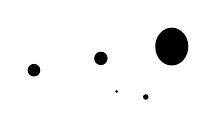
\begin{tikzpicture}[x=1cm,y=1cm]
\fill (0,0) circle (.08);
\fill (.85,.15) circle (.085);
\fill (1.75,.3) ellipse (.21 and .24);
\fill (1.05,-.27) circle (.018);
\fill (1.42,-.34) circle (.035);
\end{tikzpicture}}
\mspage{27}
